\chapter{Multivariable calculus done correctly}
As I have ranted about before, linear algebra is done wrong
by the extensive use of matrices to obscure the structure of a linear map.
Similar problems occur with multivariable calculus, so here I would like to set 
the record straight.

Since we are doing this chapter using morally correct linear algebra,
it's imperative you're comfortable with linear maps,
and in particular the dual space $V^\vee$ which we will repeatedly use.

In this chapter, all vector spaces have norms and finite-dimensional over $\RR$.

\section{The total derivative}
\prototype{If $f(x,y) = x^2+y^2$, then $(Df)_{(x,y)} = 2x\ee_1^\vee + 2y\ee_2^\vee$.}
First, let $f : [a,b] \to \RR$.
You might recall from high school calculus that for every point $p \in \RR$,
we defined $f'(p)$ as the derivative at the point $p$ (if it existed), which we interpreted as the \emph{slope} of
the ``tangent line''.

\begin{center}
	\begin{asy}
		import graph;
		size(150,0);

		real f(real x) {return 3-2/(x+2.5);}
		graph.xaxis("$x$");
		graph.yaxis();
		draw(graph(f,-2,2,operator ..), heavygray, Arrows);

		real p = -1;
		real h = 1000 * (f(p+0.001)-f(p));
		real r = 0.9;
		draw( (p+r,f(p)+r*h)--(p-r,f(p)-r*h), red);
		dot( (p, f(p)) );
		draw( (p, f(p))--(p,0), dashed);
		dot("$p$", (p, 0), dir(-90));
		label("$f'(p)$", (p+r/2, f(p) + h*r/2), dir(115));
	\end{asy}
\end{center}

That's fine, but I claim that the ``better'' way to interpret
the derivative at that point is as a \emph{linear map},
that is, as a \emph{function}.
If $f'(p) = 1.5$,
then the derivative tells me that if I move $\eps$ away from $p$
then I should expect $f$ to change by about $1.5\eps$.
In other words,
\begin{moral}
The derivative of $f$ at $p$ approximates $f$ near $p$ by a \emph{linear function}.
\end{moral}

What about more generally?
Suppose I have a function like $f : \RR^2 \to \RR$, say 
\[ f(x,y) = x^2+y^2 \]
for concreteness or something.
For a point $p \in \RR^2$, the ``derivative'' of $f$ at $p$ ought to represent a linear map
that approximates $f$ at that point $p$.
That means I want a linear map $T : \RR^2 \to \RR$ such that
\[ f(p + v) \approx f(p) + T(v) \]
for small displacements $v \in \RR^2$.

Even more generally, if $f : U \to W$ with $U \subseteq V$ open,
then the derivative at $p \in U$ ought to be so that
\[ f(p + v) \approx f(p) + T(v) \in W. \]
(We need $U$ open so that for small enough $v$, $p+v \in U$ as well.)
In fact this is exactly what we're doing earlier with $f'(p)$ in high school.

\begin{center}
	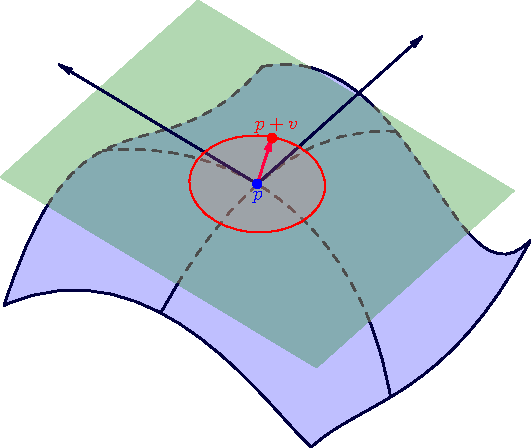
\includegraphics{media/tangent.pdf}
	\\ \tiny Image derived from \cite{img:tangentplane}
\end{center}


The only difference is that, by an unfortunate coincidence,
a linear map $\RR \to \RR$ can be represented by just its slope.
And in the unending quest to make everything a number so that it can be AP tested,
we immediately forgot all about what we were trying to do in the first place
and just defined the derivative of $f$ to be a \emph{number} instead of a \emph{function}.

\begin{moral}
	The fundamental idea of Calculus is the local approximation of functions by linear functions.
	The derivative does exactly this.
\end{moral}
Jean Dieudonn\'e as quoted in \cite{ref:pugh} continues:
\begin{quote}
	In the classical teaching of Calculus, this idea is immediately obscured
	by the accidental fact that, on a one-dimensional vector space,
	there is a one-to-one correspondence between linear forms and numbers,
	and therefore the derivative at a point is defined as a number instead of a linear form.
	This \textbf{slavish subservience to the shibboleth of numerical interpretation at any cost}
	becomes much worse . . .
\end{quote}

So let's do this right.
The only thing that we have to do is say what ``$\approx$'' means, and for
this we use the norm of the vector space.
\begin{definition}
	Let $U \subseteq V$ be open.
	Let $f : U \to W$ be a continuous function, and $p \in U$.
	Suppose there exists a linear map $T : V \to W$ such that
	\[
		\lim_{\norm{v} \to 0}
		\frac{\norm{f(p + v) - f(p) - T(v)}_W}{\norm{v}_V} = 0.
	\]
	Then $T$ is the \vocab{total derivative} of $f$ at $p$.
	We denote this by $(Df)_p$, and say $f$ is \vocab{differentiable at $p$}.

	If $(Df)_p$ exists at every point, we say $f$ is \vocab{differentiable}.
\end{definition}

\begin{ques}
	Check if that $V = W = \RR$, this is equivalent to the single-variable definition.
	(What are the linear maps from $V$ to $W$?)
\end{ques}
\begin{example}[Total derivative of $f(x,y) = x^2+y^2$]
	Let $V = \RR^2$ with standard basis $\ee_1$, $\ee_2$ and let $W = \RR$,
	and let $f\left( x \ee_1 + y \ee_2 \right) = x^2+y^2$.  Let $p = a\ee_1 + b\ee_2$.
	Then, we claim that \[ (Df)_p : \RR^2 \to \RR \quad\text{by}\quad
	v \mapsto 2a \cdot \ee_1^\vee(v) + 2b \cdot \ee_2^\vee(v). \]
\end{example}
Here, the notation $\ee_1^\vee$ and $\ee_2^\vee$ makes sense,
because by definition $(Df)_p \in V^\vee$: these are functions from $V$ to $\RR$!

Let's check this manually with the limit definition.
Set $v = xe_1 + ye_2$, and note that the norm on $V$ is $\norm{(x,y)}_V = \sqrt{x^2+y^2}$
while the norm on $W$ is just the absolute value $\norm{c}_W = \left\lvert c \right\rvert$.
Then we compute
\begin{align*}
	\frac{\norm{f(p + v) - f(p) - T(v)}_W}{\norm{v}_V} 
	&= \frac{\left\lvert (a+x)^2 + (b+y)^2 - (a^2+b^2) - (2ax+2by) \right\rvert}{\sqrt{x^2+y^2}} \\
	&= \frac{x^2+y^2}{\sqrt{x^2+y^2}} = \sqrt{x^2+y^2} \\
	&\to 0
\end{align*}
as $\norm{v} \to 0$.
Thus, for $p = ae_1 + be_2$ we indeed have $(Df)_p = 2a \cdot e_1^\vee + 2b \cdot e_2^\vee$.

\begin{remark}
	As usual, differentiability implies continuity.
\end{remark}
\begin{remark}
	Although $U \subseteq V$, it might be helpful to think of vectors from $U$ and $V$
	as different types of objects (in particular, note that it's possible for $0_V \notin U$).
	The vectors in $U$ are ``inputs'' on our space
	while the vectors coming from $V$ are ``small displacements''.
	For this reason, I deliberately try to use $p \in U$ and $v \in V$ when possible.
\end{remark}

\section{The projection principle}
Before proceeding I need to say something really important.
\begin{theorem}[Projection principle]
	\label{thm:project_principle}
	Let $W$ be an $n$-dimensional real vector space with basis $w_1, \dots, w_n$.
	Then there is a bijection between continuous functions $f : U \to W$ and
	$n$-tuples of continuous $f_1, f_2, \dots, f_n : U \to \RR$
	by projection onto the $i$th basis element, i.e.\ 
	\[ f(v) = f_1(v)w_1 + \dots + f_n(v)w_n. \]
\end{theorem}
\begin{proof}
	Obvious.
\end{proof}
The theorem remains true if one replaces ``continuous'' by ``differentiable'', ``smooth'', ``arbitrary'',
or most other reasonable words. Translation:
\begin{moral}
To think about a function $f : U \to \RR^{n}$,
it suffices to think about each coordinate separately.
\end{moral}
For this reason, we'll most often be interested in functions $f : U \to \RR$.
That's why the dual space $V^\vee$ is so important.

\section{Total and partial derivatives}
\prototype{If $f(x,y) = x^2+y^2$, then $(Df) : (x,y) \mapsto 2x\ee_1^\vee + 2y\ee_2^\vee$, and
$\fpartial fx = 2x$, $\fpartial fy = 2y$.}
Let $U \subseteq V$ be open and let $V$ have a basis $e_1$, \dots, $e_n$.
Suppose $f : U \to \RR$ is a function which is differentiable everywhere,
meaning $(Df)_p \in V^\vee$ exists for every $p$.
In that case, one can consider $Df$ as \emph{itself} a function:
\begin{align*}
	Df : U &\to V^\vee \\
	p &\mapsto (Df)_p.
\end{align*}
This is a little crazy: to every \emph{point} in $U$ we associate a \emph{function} in $V^\vee$.
We say $Df$ is the \vocab{total derivative} of $f$ at $p$,
to reflect how much information we're dealing with.

Let's apply the projection principle now to $Df$.
Since we picked a basis $e_1$, \dots, $e_n$ of $V$,
there is a corresponding dual basis
$e_1^\vee$, $e_2^\vee$, \dots, $e_n^\vee$.
The Projection Principle tells us that $Df$ can thus be thought of as just $n$ functions, so we can write
\[ Df = \psi_1 e_1^\vee + \dots + \psi_n e_n^\vee.  \]
In fact, we can even describe what the $\psi_i$ are.
\begin{definition}
	The \vocab{$i^{\text{th}}$ partial derivative} of $f : U \to \RR$, denoted 
	\[ \fpartial{f}{e_i}: U \to \RR \]
	is defined by
	\[
		\fpartial{f}{e_i} (p)
		\defeq \lim_{t \to 0} \frac{f(p + te_i) - f(p)}{t}.
	\]
\end{definition}
You can think of it as ``$f'$ along $e_i$''.
\begin{ques}
	Check that if $Df$ exists, then \[ (Df)_p(e_i) = \fpartial{f}{e_i}(p). \]
\end{ques}
\begin{remark}
	Of course you can write down a definition of $\fpartial{f}{v}$
	for any $v$ (rather than just the $e_i$).
\end{remark}

From the above remarks, we can derive that
\[
	\boxed{
	Df =
	\frac{\partial f}{\partial e_1} \cdot e_1^\vee
	+ \dots + 
	\frac{\partial f}{\partial e_n} \cdot e_n^\vee .
	}
\]
and so given a basis of $V$, we can think of $Df$ as just
the $n$ partials.
\begin{remark}
Keep in mind that each $\frac{\partial f}{\partial e_i}$ is a function from $U$ to the \emph{reals}.
That is to say,
\[
	(Df)_p =
	\underbrace{\frac{\partial f}{\partial e_1}(p)}_{\in \RR} \cdot e_1^\vee
	+ \dots + 
	\underbrace{\frac{\partial f}{\partial e_n}(p)}_{\in \RR} \cdot e_n^\vee
	\in V^\vee.
\]
\end{remark}


\begin{example}[Partial derivatives of $f(x,y) = x^2+y^2$]
	Let $f : \RR^2 \to \RR$ by $(x,y) \mapsto x^2+y^2$.
	Then in our new language, 
	\[ Df : (x,y) \mapsto 2x \cdot \ee_1^\vee + 2y \cdot \ee_2^\vee. \]
	Thus the partials are
	\[
		\frac{\partial f}{\partial x} : (x,y) \mapsto 2x \in \RR
		\quad\text{and}\quad
		\frac{\partial f}{\partial y} : (x,y) \mapsto 2y \in \RR
	\]
\end{example}

With all that said, I haven't really said much about how to
find the total derivative itself.
For example, if I told you
\[ f(x,y) = x \sin y + x^2y^4 \]
you might want to be able to compute $Df$ without going through
that horrible limit definition I told you about earlier.

Fortunately, it turns out you already know how to compute partial derivatives,
because you had to take AP Calculus at some point in your life.
It turns out for most reasonable functions, this is all you'll ever need.
\begin{theorem}[Continuous partials implies differentiable]
	Let $U \subseteq V$ be open and pick any basis $e_1, \dots, e_n$.
	Let $f : U \to W$ and suppose that $\fpartial{f}{e_i}$ is defined
	for each $i$ and moreover is \emph{continuous}.
	Then $f$ is differentiable and given by
	\[ Df = \sum \fpartial{f}{e_i} \cdot e_i^\vee. \]
\end{theorem}
\begin{proof}
	Not going to write out the details, but\dots
	given $v = t_1e_1 + \dots + t_ne_n$,
	the idea is to just walk from $p$ to $p+t_1e_1$, $p+t_1e_1+t_2e_2$, \dots,
	up to $p+t_1e_1+t_2e_2+\dots+t_ne_n = p+v$,
	picking up the partial derivatives on the way.
	Do some calculation.
\end{proof}

\begin{remark}
	The continuous condition cannot be dropped. The function
	\[
			f(x,y)
		=
		\begin{cases}
			\frac{xy}{x^2+y^2} & (x,y) \neq (0,0) \\
			0 & (x,y) = (0,0).
		\end{cases}
	\]
	is the classic counterexample -- the total derivative $Df$ does not exist at zero,
	even though both partials do.
\end{remark}

\begin{example}
	[Actually computing a total derivative]
	Let $f(x,y) = x \sin y + x^2y^4$. Then
	\begin{align*}
		\fpartial fx (x,y) &= \sin y + y^4 \cdot 2x \\
		\fpartial fy (x,y) &= x \cos y + x^2 \cdot 4y^3.
	\end{align*}
	Then $Df = \fpartial fx \ee_1^\vee + \fpartial fy \ee_2^\vee$,
	which I won't bother to write out.
\end{example}

The example $f(x,y) = x^2+y^2$ is the same thing.
That being said, who cares about $x \sin y + x^2y^4$ anyways?

\section{(Optional) A word on higher derivatives}
Let $U \subseteq V$ be open, and take $f : U \to W$, so that $Df : U \to \Hom(V,W)$.

Well, $\Hom(V,W)$ can also be thought of as a normed vector space in its own right:
it turns out that one can define an operator norm on it by setting
\[ \norm{T} \defeq \sup \left\{ \frac{\norm{T(v)}_W}{\norm{v}_W} \mid v \neq 0_V \right\}. \] 
So $\Hom(V,W)$ can be thought of as a normed vector space as well.
Thus it makes sense to write
\[ D(Df) : U \to \Hom(V,\Hom(V,W)) \]
which we abbreviate as $D^2 f$. Dropping all doubt and plunging on,
\[ D^3f : U \to \Hom(V, \Hom(V,\Hom(V,W))). \]
I'm sorry.
As consolation, we at least know that $\Hom(V,W) \cong V^\vee \otimes W$ in a natural way,
so we can at least condense this to
\[ D^kf : V \to (V^\vee)^{\otimes k} \otimes W \]
rather than writing a bunch of $\Hom$'s.
\begin{remark}
	If $k=2$, $W = \RR$, then $D^2f(v) \in (V^\vee)^{\otimes 2}$,
	so it can be represented as an $n \times n$ matrix,
	which for some reason is called a \vocab{Hessian}.
\end{remark}
The most important property of the second derivative is that
\begin{theorem}
	[Symmetry of $D^2 f$]
	Let $f : U \to W$ with $U \subseteq V$ open.
	If $(D^2f)_p$ exists at some $p \in U$, then it is symmetric, meaning
	\[ (D^2f)_p(v_1, v_2) = (D^2f)_p(v_2, v_1). \]
\end{theorem}
I'll just quote this without proof (see e.g. \cite[\S5, theorem 16]{ref:pugh}),
because double derivatives make my head spin.
An important corollary of this theorem:
\begin{corollary}
	[Clairaut's theorem: mixed partials are symmetric]
	Let $f : U \to \RR$ with $U \subseteq V$ open be twice differentiable.
	Then for any point $p$ such that the quantities are defined,
	\[
		\frac{\partial}{\partial e_i}
		\frac{\partial}{\partial e_j}
		f(p)
		=
		\frac{\partial}{\partial e_j}
		\frac{\partial}{\partial e_i}
		f(p).
	\]
\end{corollary}

\section{Towards differential forms}
This concludes the exposition of what the derivative really is:
the key idea I want to communicate in this chapter is that $Df$
should be thought of as a map from $U \to V^\vee$.

The next natural thing to do is talk about \emph{integration}.
The correct way to do this is through a so-called \emph{differential form}:
you'll finally know what all those stupid $dx$'s and $dy$'s really mean.
(They weren't just there for decoration!)

\section\problemhead
\begin{sproblem}[Chain rule]
	Let $U_1 \taking f U_2 \taking g U_3$ be differentiable maps
	between open sets of normed vector spaces $V_i$, and let $h = g \circ f$.
	Prove the Chain Rule: for any point $p \in U_1$, we have
	\[ (Dh)_p = (Dg)_{f(p)} \circ (Df)_p. \]
\end{sproblem}

\begin{problem}
	Let $U \subseteq V$ be open, and $f : U \to \RR$ be differentiable $k$ times.
	Show that $(D^kf)_p$ is symmetric in its $k$ arguments, meaning for any $v_1, \dots, v_k \in V$
	and any permutation $\sigma$ on $\left\{ 1, \dots, k \right\}$ we have
	\[ (D^kf)_p(v_1, \dots, v_k) = (D^kf)_p(v_{\sigma(1)}, \dots, v_{\sigma(k)}). \]
	\begin{hint}
		Simply induct, with the work having been done on the $k=2$ case.
	\end{hint}
\end{problem}
